\chapter{考察}
\par
本実験の結果,MIoM SCAINは信念と欲求の推定の両方においてUIoM SCAIN (action)およびUIoM SCAIN (utterance)よりも強い相関を示した.信念推定および欲求推定においてMIoM SCAINがUIoM SCAIN (aciton)やUIoM SCAIN (utterance)より強い相関を示した要因の一つとして,MIoM SCAINが散策行動情報と人間の発話情報の両方を信念と欲求の推定に反映していることが考えられる.本実験における設定では,散策行動情報と人間の発話情報の両方が観測される設定であり,人間の発話情報から散策行動情報の解釈が変わったり,散策行動情報から人間の発話情報の解釈が変わることがあった.例えば,図\ref{fig:ex_env2}が示すような場合を考える.
\begin{figure}[htbp]
  \begin{center}
    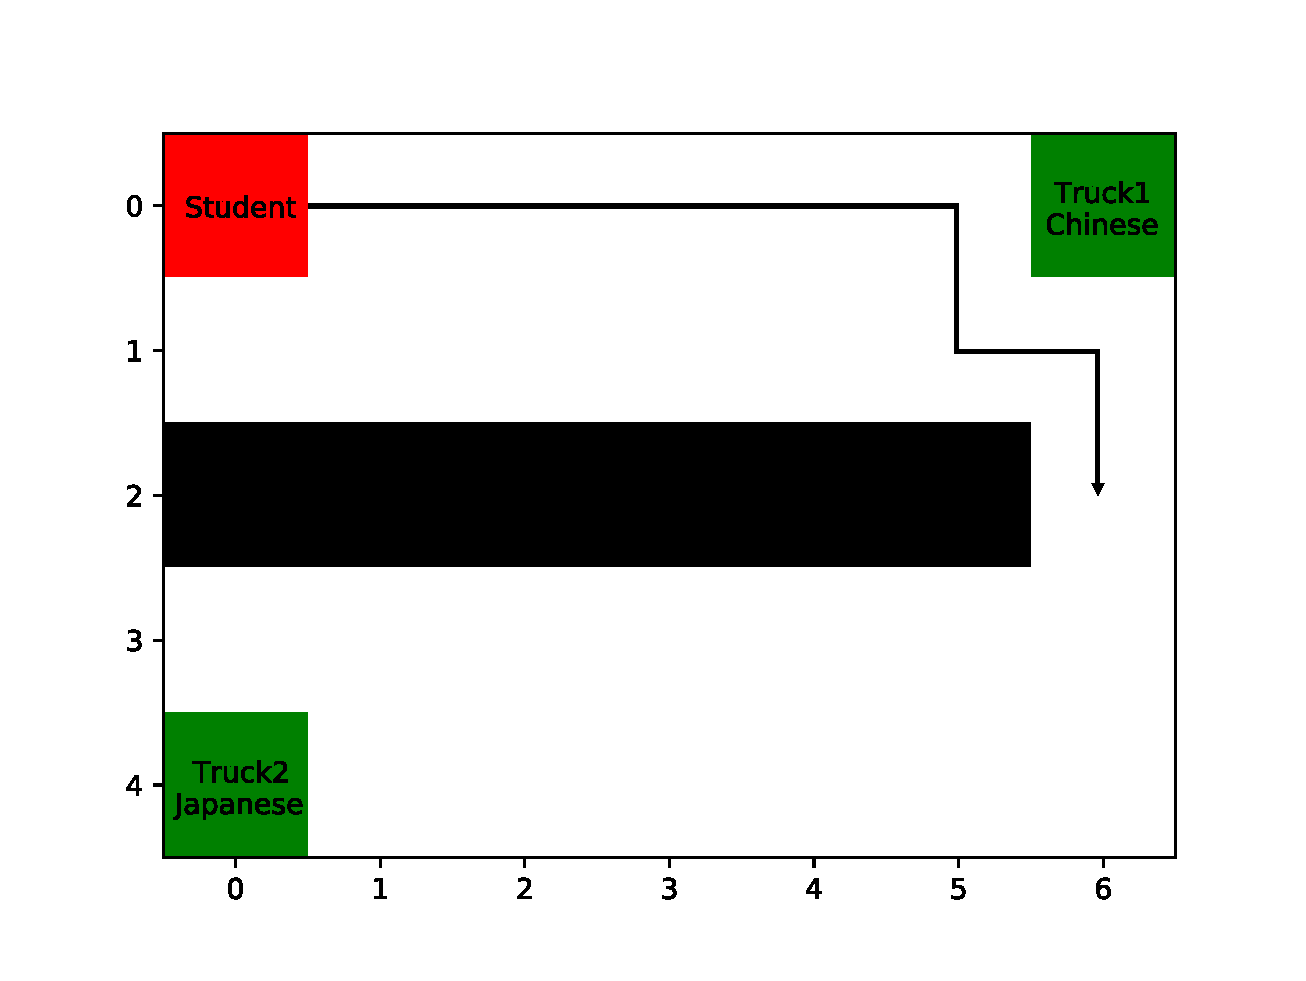
\includegraphics[scale=0.48]{./ex_env2.pdf}
    \caption{学生がTruck1を通過した場面}
    \label{fig:ex_env2}
  \end{center}
\end{figure}
この場合,散策行動情報のみに基づいて学生の散策行動を解釈すると,学生はTruck2に向かっていると解釈することができる.しかし「こってりした料理を食べたい」という学生発話情報が観測された時,発話情報も考慮して学生の散策行動を解釈すると,学生は単に屋台の種類を確認するためにTruck2に向かっていると解釈することができる.また,「こってり料理を食べたい」という学生の発話情報が観測された時,発話情報のみに基づいて学生の発話文を解釈すると,イタリア料理や中華料理について言及していると解釈することができる.しかし図\ref{fig:ex_env2}が示す散策行動情報が観測された時,散策行動情報も考慮して学生の発話文を解釈すると,学生の発話文はこってりした日本食を食べたいということを表していると解釈することができる.
MIoM SCAINは,人間の発話情報による散策行動情報の解釈の決定や散策行動情報による人間の発話情報の解釈の決定を行い,散策行動情報と人間の発話情報の相互依存を推定に反映することでUIoM SCAINの推定結果を上回ったと考えられる.MIoM SCAINの推定により,信念と欲求の推定において散策行動情報と人間の発話情報を両方用いることが有効であると考えられる.

\par
また,本実験では3つの推定システムにおいて欲求推定の相関が信念推定の相関より強いことが示された.そこで本実験で用いた3つの推定システムにおいて欲求推定が信念推定よりも強い相関を示した要因を考える.実験参加者による推定結果を分析したところ,欲求推定では散策行動情報と学生の発話情報の両方が大きく影響していたが,信念推定では学生の発話情報の影響が大きいことがわかった.例えば,図\ref{fig:ex_env2}に示すように,Truck1は観測しているがTruck2を観測していない状況でTruck1からは遠ざかりTruck2に向かう状況を考える.
この時,Truck2に向かっているという散策行動情報は信念の推定に活用することは困難であり,Truck1での食事よりもTruck2での食事を好んでいる可能性が高いという欲求の推定にのみ大きく影響することが考えられる.そのため,実験参加者による信念の推定では学生の発話情報からの影響が大きくなったと考えられる.
しかし学生の発話情報は欲求を問うものが多かったため,学生の発話情報が信念推定に大きな影響を与えることができても,信念の正確な推定に寄与することが困難であったと考える.本実験では,表\ref{tab:q_a}の学生の応答を発話情報として採用している.表\ref{tab:q_a}からわかるように,学生の発話情報は欲求に関する内容である.そのため,学生の発話情報は信念推定および欲求推定に大きい影響を与え,欲求推定の性能向上を寄与することができても,信念推定の性能向上に寄与することはできないと考える.このような理由から,信念推定において信念を問う学生の発話情報を増やすことが有効であると考えられる.
